\let\negmedspace\undefined
\let\negthickspace\undefined
\documentclass[journal,12pt,onecolumn]{IEEEtran}
\usepackage{cite}
\usepackage{amsmath,amssymb,amsfonts,amsthm}
\usepackage{algorithmic}
\usepackage{graphicx}
\graphicspath{{./figs/}}
\usepackage{textcomp}
\usepackage{xcolor}
\usepackage{txfonts}
\usepackage{listings}
\usepackage{enumitem}
\usepackage{mathtools}
\usepackage{gensymb}
\usepackage{comment}
\usepackage{caption}
\usepackage[breaklinks=true]{hyperref}
\usepackage{tkz-euclide} 
\usepackage{listings}
\usepackage{gvv}                                        
%\def\inputGnumericTable{}                                 
\usepackage[latin1]{inputenc}     
\usepackage{xparse}
\usepackage{color}                                            
\usepackage{array}
\usepackage{longtable}                                       
\usepackage{calc}                                             
\usepackage{multirow}
\usepackage{multicol}
\usepackage{hhline}                                           
\usepackage{ifthen}                                           
\usepackage{lscape}
\usepackage{tabularx}
\usepackage{array}
\usepackage{float}
\newtheorem{theorem}{Theorem}[section]
\newtheorem{problem}{Problem}
\newtheorem{proposition}{Proposition}[section]
\newtheorem{lemma}{Lemma}[section]
\newtheorem{corollary}[theorem]{Corollary}
\newtheorem{example}{Example}[section]
\newtheorem{definition}[problem]{Definition}
\newcommand{\BEQA}{\begin{eqnarray}}
\newcommand{\EEQA}{\end{eqnarray}}
\newcommand{\define}{\stackrel{\triangle}{=}}
\theoremstyle{remark}
\newtheorem{rem}{Remark}

\begin{document}

\title{12.693}
\author{ee25btech11056 - Suraj.N}
\maketitle
\renewcommand{\thefigure}{\theenumi}
\renewcommand{\thetable}{\theenumi}

\begin{document}

\textbf{Question :} Suppose the circles 

\begin{align*}
x^2 + y^2 + ax + 6 &= 0 \\
x^2 + y^2 + bx - 4 &= 0
\end{align*}
intersect each other orthogonally at the point $(1,2)$. Then $a+b = \_$

\textbf{Solution :}

\begin{table}[h!]
  \centering
  \begin{tabular}{|c|c|}
\hline
\textbf{Name} & \textbf{Value} \\ \hline
$\vec{A}$ & $\myvec{2 & 1 \\0 & 3}$ \\ \hline
\end{tabular}

  \caption*{Table : Circles and Point}
  \label{12.693}
\end{table}

The conic parameters for the two circles can be expressed as :

\begin{align}
  \vec{V_1} &= \vec{I} & \vec{u_1} &= \myvec{\tfrac{a}{2} \\0 } & f1 &= 6\\
  \vec{V_2} &= \vec{I} & \vec{u_2} &= \myvec{\tfrac{b}{2} \\ 0} & f2 &= -4
\end{align}

The point of intersection of the two circles is $\vec{P}$\\

The equation of tangent to Circle 1 at $\vec{P}$ is given as :

\begin{align}
  (\vec{V_1}\vec{P}+\vec{u_1})^\top\vec{x} + \vec{u_1}^\top\vec{P} + f_1 &= 0 & \vec{n_1} &= \vec{V_1}\vec{P}+\vec{u_1} 
\end{align}

The equation of tangent to Circle 2 at $\vec{P}$ is given as :

\begin{align}
  (\vec{V_2}\vec{P}+\vec{u_2})^\top\vec{x} + \vec{u_2}^\top\vec{P} + f_2 &= 0 & \vec{n_2} &= \vec{V_2}\vec{P}+\vec{u_2} 
\end{align}

As the tangents at $\vec{P}$ are perpendicular , the normal vectors of the tangents are also perpendicular 

\begin{align}
  \vec{n_1}^\top\vec{n_2} = 0\\
  (\vec{V_1}\vec{P}+\vec{u_1})^\top(\vec{V_2}\vec{P}+\vec{u_2}) = 0\\
  (\vec{P}+\vec{u_1})^\top(\vec{P}+\vec{u_2}) = 0\\
  (\vec{P}^\top+\vec{u_1}^\top)(\vec{P}+\vec{u_2}) = 0 \label{eq:tangent} \\
  \myvec{\tfrac{a+2}{2} & 2}\myvec{\tfrac{b+2}{2}\\2} = 0\\
  2(a+b) + ab + 20 = 0  \label{eq:a+b} 
\end{align}

\pagebreak

As $\vec{P}$ lies on both the circles we get :

\begin{align}
  \vec{P}^\top \vec{P} + 2\vec{u_1}^\top \vec{P} + f_1 = 0 \label{eq:circle1} \\
  \vec{P}^\top \vec{P} + 2\vec{u_2}^\top \vec{P} + f_2 = 0 
\end{align}

By subtracting the above two equations we get :

\begin{align}
  (\vec{u_1}^\top - \vec{u_2}^\top)\vec{P} = \frac{f_2 - f_1}{2} \label{eq:p1} 
\end{align}

If we substitue \eqref{eq:circle1} in \eqref{eq:tangent} we get :

\begin{align}
  (\vec{u_2}^\top - \vec{u_1}^\top)\vec{P} + \vec{u_1}^\top\vec{u_2} - f_1 = 0\\
  (\vec{u_1}^\top - \vec{u_2}^\top)\vec{P} = \vec{u_1}^\top\vec{u_2} - f_1   \label{eq:p2} 
\end{align}

From \eqref{eq:p1} and \eqref{eq:p2} , we get :

\begin{align}
  \vec{u_1}^\top\vec{u_2} = \frac{f_1+f_2}{2}\\
  ab = 4  \label{eq:ab}
\end{align}

By substituting \eqref{eq:ab} in \eqref{eq:a+b} , we get :

\begin{align}
a + b = -12
\end{align}

\pagebreak

\begin{figure}[h!]
  \centering
  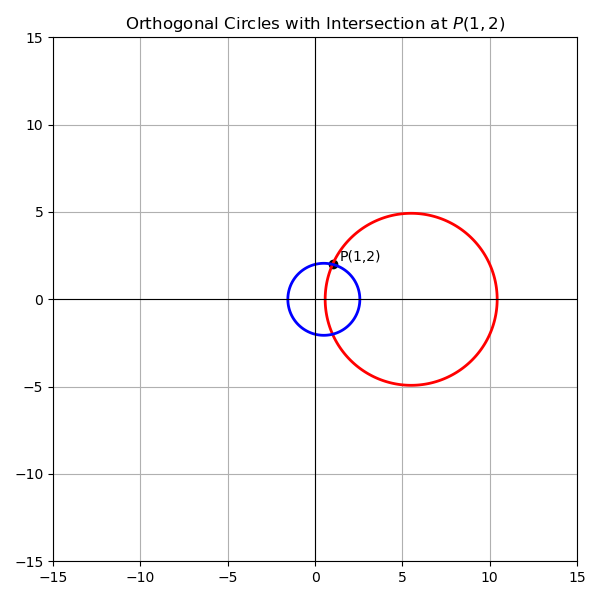
\includegraphics[width=0.7\columnwidth]{figs/circles.png} 
   \caption*{Fig : Circles}
  \label{Fig1}
\end{figure}

\end{document}
